\chapter{证明器的总体设计}
\label{chap:struct}

\section{设计目标}
支持分离逻辑
支持证明项构造
支持等词和未解释函数
支持线性整数理论
\section{输入语言}

\begin{figure}[!htbp]
  \centering
  \begin{tabular}[rcl]{rcl}
    $E$ & \sep{} & $x$ \deli{} $a$ \deli{} $f_i(E,$\ldots$,E)$ \deli{} $+(E, E)$ \deli{} $.(a,E)$ \\
    $T$ & \sep{} & $E \le E$ \deli{} $E = E$ \deli{} $A$ \\
    $\Pi$ & \sep{} & $T$ \deli{}  $\lnot \Pi$ \deli{} $\Pi \impl \Pi$ \deli{} $\Pi \land \Pi$ \deli{} $\Pi \lor \Pi$ \\
    $\Sigma$ & \sep{} & $E \mapsto E$ \deli{} $\Sigma \ast \Sigma$ \\
    $\Delta$ & \sep{} & $\Sigma \land \Pi$ \\
  \end{tabular}
\end{figure}


\section{结构框图}

\begin{figure}[!htbp]
  \centering
  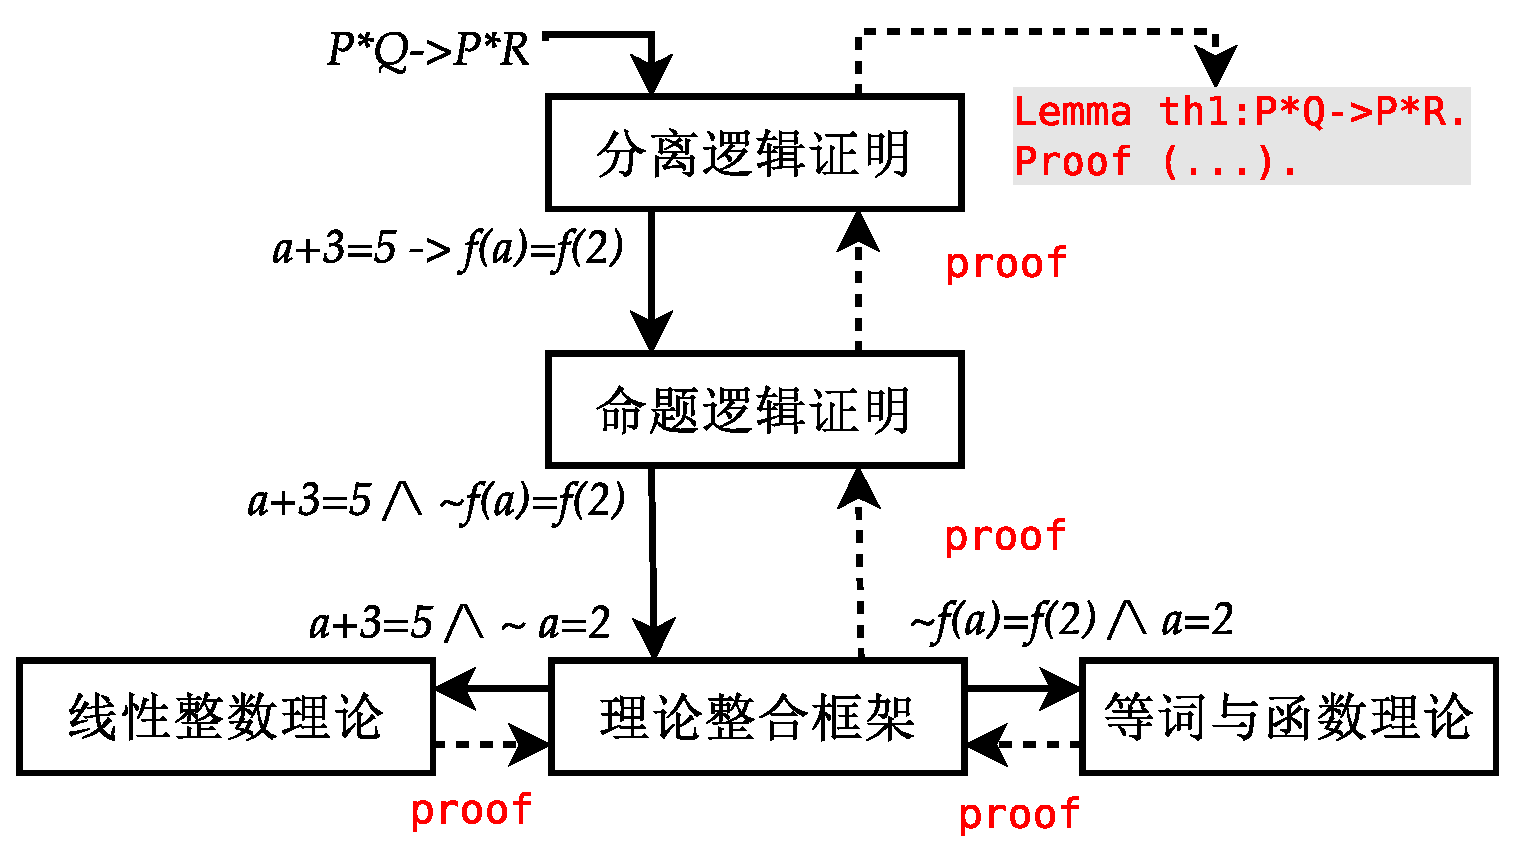
\includegraphics[width=0.9\textwidth]{stru.eps}
\end{figure}

\section{工作原理}

